\documentclass{article}
\usepackage[german]{babel}
\usepackage{float}
\usepackage{fourier}
\usepackage[utf8]{inputenc}
\usepackage[T1]{fontenc}
\usepackage{amsfonts,amsthm, amsmath}
\usepackage{listings}
% The following is needed in order to make the code compatible
% with both latex/dvips and pdflatex.
\ifx\pdftexversion\undefined
\usepackage[dvips]{graphicx}
\else
\usepackage[pdftex]{graphicx}
\DeclareGraphicsRule{*}{mps}{*}{}
\fi

\setlength\parindent{0pt}
\lstset{language=Java}

\begin{document}

\textbf{Team:} TEAM 01, Falco Winkler (FW), Daniel Schruhl (DS)\\
\\
\textbf{Aufgabenteilung:}
\begin{itemize}
    \item IDL Compiler (FW)
    \item Namensdienst (DS)
    \item mware\_lib Library (FW,DS)
\end{itemize}

\textbf{Quellenangaben:}
\begin{itemize}
    \item Aufgabe 4, 11.06.2017, C. Klauck \& H. Schulz: \newline
    http://users.informatik.haw-hamburg.de/~schulz/pub/Verteilte-Systeme/AI5-VSP/Aufgabe4/
\end{itemize}

\textbf{Bearbeitungszeitraum:}
\begin{itemize}
	\item 11.06.2017 4 Stunden (DS,FW)
	\item 12.06.2017 2 Stunden (DS)
	\item 12.06.2017 3 Stunden (FW)
	\item 14.06.2017 4 Stunden (DS)
	\item 14.06.2017 5 Stunden (FW)
	\item 15.06.2017 5 Stunden (DS)
	\item 16.06.2017 5 Stunden (DS)
\end{itemize}

\textbf{Aktueller Stand:}
\begin{itemize}
	\item IDL Compiler fertig und getestet
    \item Namensdienst fertig und getestet
    \item mware\_lib Library fertig
\end{itemize}

\textbf{Änderung des Entwurfs:}
\begin{itemize}
    \item Protokolle in extra Kapitel genauer beschrieben
\end{itemize}

\newpage

\section{Einführung und Ziele}
Es soll eine einfache objektorientierte Middleware entworfen werden, die Methodenaufrufe
eines entfernten Objektes ermöglicht.\\

Zur Orientierung gilt hierbei die CORBA Architektur. Genauer soll hier ein ORB zur
Verfügung gestellt werden, der es ermöglicht Methoden von entfernten Objekten aufzurufen.\\

Zur Abstraktion und Beschreibung der Schnittstellen der Objekte soll eine IDL verwendet werden.
Diese IDL wird dann zur Erzeugung von Klassen- und Methodenrümpfen verwendet.\\

Außerdem beinhaltet der ORB einen Namensdienst, der Objektreferenzen in einem Netz mit Namen finden
kann.\\

Die Middleware an sich soll durch eine Library abstrahiert und verwendbar sein.

\subsection{Randbedingungen}
Der Namensdienst soll auf einem entfernten Rechner unabhängig von der Middleware Library
lauffähig sein. Der Port muss zur Laufzeit einstellbar sein.\\

Der IDL-Compiler soll in einem Package oder einer \texttt{.jar} Datei zur Verfügung gestellt
werden. Der Compiler soll folgende IDL Typen unterstützen:

\begin{itemize}
    \item module (keine Schachtelung, 1 Modul pro Datei)
    \item class (nicht als Parameter oder Returnwert, keine Schachtelung)
    \item int
    \item double
    \item string
\end{itemize}

Ein Beispiel:
\begin{lstlisting}
module math_ops {
  class Calculator {
   double add(double a, double b);
   string getStr(double a);
 };
};
\end{lstlisting}

Die Middleware Library soll in einem Package \texttt{mware\_lib} zusammengefasst werden.\\

Wenn eine Serverapplikation während eines entfernten Methodenaufrufes eine RuntimeException
wirft, soll diese an den Aufrufer weitergeleitet werden.\\

Es soll möglich sein, dass zwei oder mehrere Klienten die selbe Objektreferenz zeitgleich
nutzen wollen. Das soll innerhalb der Middleware nicht zu Deadlocks führen.

\subsection{Kontextbegrenzung}
Die Implementierung soll in Java vorliegen.

Die Behebung von Deadlocks in den Anwendungen ist nicht Aufgabe der Middleware.

\newpage

\section{Gesamtsystem}
Das Gesamtsystem besteht aus drei Subsystemen, die unabhängig voneinander lauffähig sind.
Dabei sind das NameService System und das IDL-Compiler System Applikationen, die über
die Kommandozeile gestartet werden können.

Die Middleware Library (mware\_lib) ist eine Bibliothek, die in der jeweiligen Applikation,
die die Middleware verwenden soll eingebunden werden muss. Die Middleware Library ist also
nicht direkt über die Kommandozeile startbar.

\subsection{Bausteinsicht}
\begin{figure}[H]
    \centering
    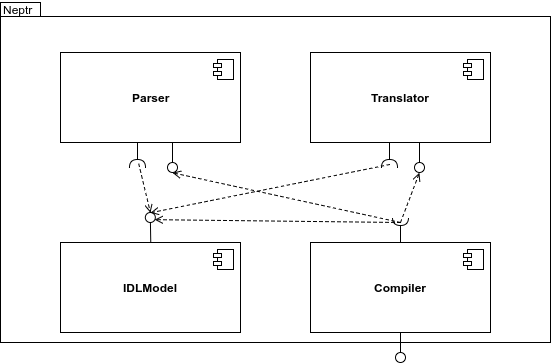
\includegraphics[width=0.8\textwidth]{compiler-components.png}
    \caption[compiler-components]{Komponentendiagramm des IDL-Compilers (Neptr)}
    \label{fig:compiler-component-diagram}
\end{figure}

\begin{figure}[H]
    \centering
    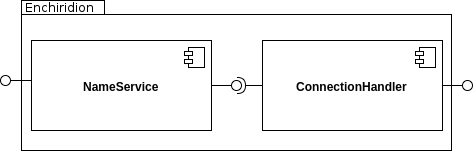
\includegraphics[width=0.6\textwidth]{nameservice-components.png}
    \caption[nameservice-components]{Komponentendiagramm des NameServices Server (Enchiridion)}
    \label{fig:nameservice-component-diagram}
\end{figure}

\begin{figure}[H]
    \centering
    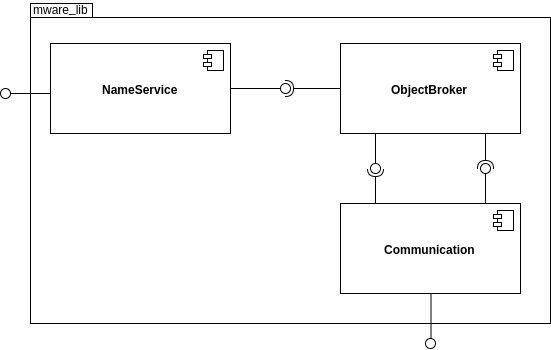
\includegraphics[width=0.7\textwidth]{Middleware_Components.png}
    \caption[middleware-components]{Komponentendiagramm der Middleware Library (mware\_lib)}
    \label{fig:middleware-components-diagram}
\end{figure}

\subsection{Laufzeitsicht}
\begin{figure}[H]
    \centering
    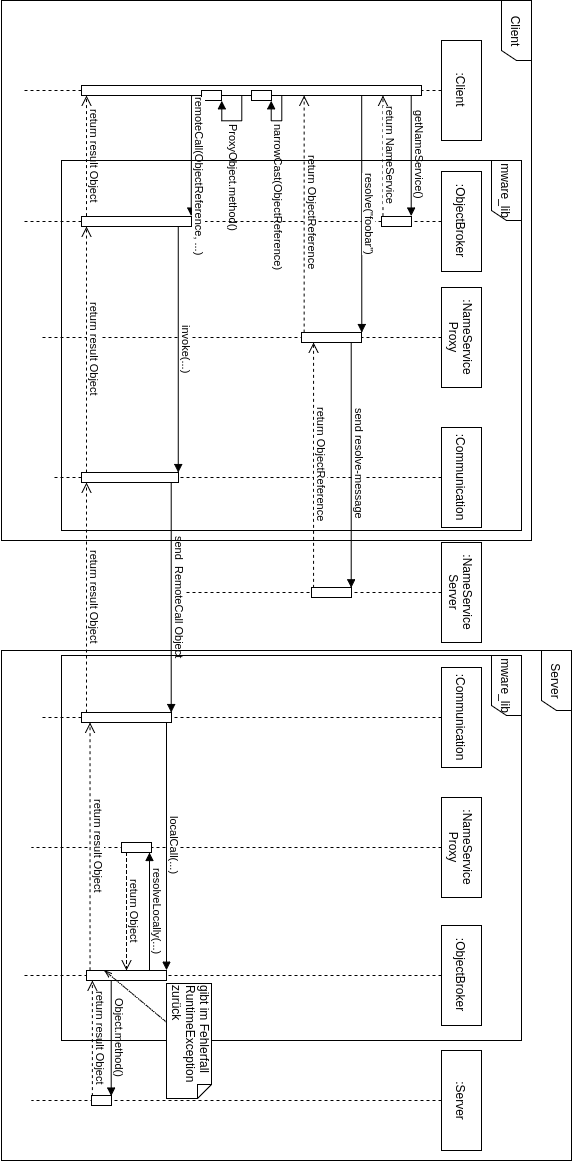
\includegraphics[width=0.7\textwidth]{full-sequence.png}
    \caption[full-seq-diagram]{Sequenzdiagramm eines entfernten Methodenaufrufes mit der Middleware}
    \label{fig:full-seq-diagram}
\end{figure}

\begin{figure}[H]
    \centering
    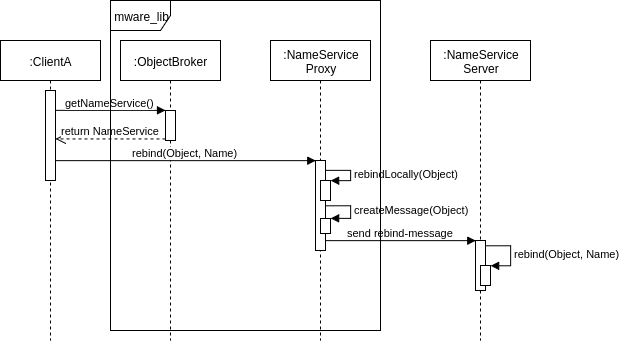
\includegraphics[width=\textwidth]{rebind-seq.png}
    \caption[rebind-seq-diagram]{Sequenzdiagramm eines Rebinds von einem Objekt}
    \label{fig:full-seq-diagram}
\end{figure}

\newpage

\section{Subsysteme und Komponenten}

\subsection{NameService (Enchiridion)}
\subsubsection{Aufgabe und Verantwortung}
Der NameService bildet Namen auf Objektreferenzen ab. Er wird verwendet, um Objekte anhand
ihres Namens zu finden und anzusprechen und um Objekte anzumelden. Er besteht dabei aus einem Client und einem Server.

\subsubsection{Schnittstelle}
Die Schnittstellen zwischen dem Client und dem Server tauschen Nachrichten per TCP mittels
u.g. Nachrichtenformat (Entwurfsentscheidungen) an gegebenem Port aus.
\begin{lstlisting}
public abstract class NameService {

    /**
     * Registers an Object (servant) at the NameService
     *
     * @param servant Object to register
     * @param name    String representation of the object
     */
    public abstract void rebind(Object servant, String name);

    /**
     * Returns the Object reference from the given servant
     *
     * @param name String of servant
     * @return general Object reference
     */
    public abstract Object resolve(String name);
}

public class NameServiceStarter {
    /**
     * Ueber die main - Methode der Klasse NameServiceStarter
     * kann der NameService (Server) gestartet werden.
     */
    public static void main(String[] args);
}
\end{lstlisting}
Zu übergebene Argumente sind:
\begin{itemize}
	\item args[0]: Port auf dem der NameService Server laufen soll
\end{itemize}

Die erzeugten Binaries können wie folgt ausgeführt werden:\\

\texttt{./bin/enchiridion <Port>}

\subsubsection{Entwurfsentscheidungen} \label{nameservice-entwurf}
\begin{figure}[H]
    \centering
    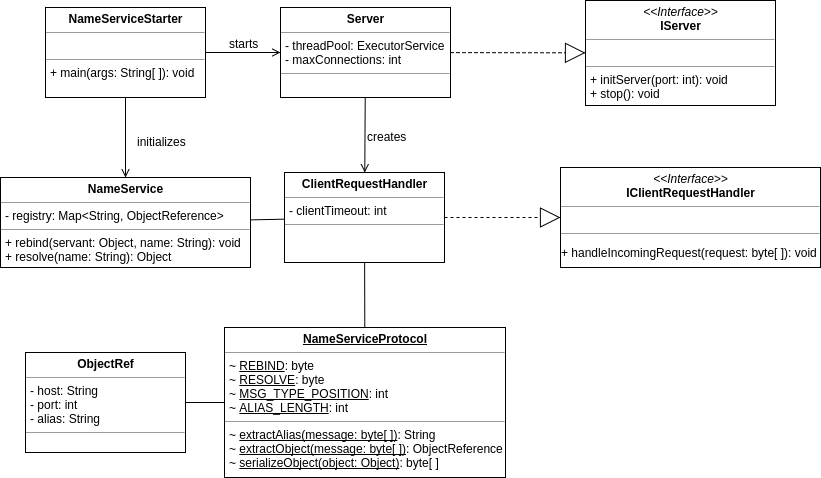
\includegraphics[width=\textwidth]{nameservice-fdm.png}
    \caption[fdm-nameservice]{Fachliches Daten Modell des NameServices}
    \label{fig:fdm-nameservice}
\end{figure}

Der NameService an sich besteht aus einem Server, der Anfragen entgegennehmen kann.
Der Client des NameServices ist in der Middleware enthalten.

Der Port, an dem der NameService läuft ist zur Laufzeit einstellbar. Das geschieht über den Startparameter.\\

Das Protokoll des Nameservice ist als seperate Bibliothek implementiert und im Abschnitt
'Protokolle' weiter beschrieben.

Der NameService besteht aus der Hauptkomponente und der ConnectionHandler Komponente (siehe Abbildung
\ref{fig:nameservice-component-diagram}).\\

Die Hauptkomponente enthält den eigentlichen NameService. Der hat eine Registry, die eine Map darstellt, in der Namen
auf Objektreferenzen abgebildet werden. Diese Registry ist threadsafe, da mehrere Clients parallel auf diese
zugreifen müssen und diese eventuell verändern können.

Der NameService an sich ist ein Singleton, wodurch sichergestellt wird, dass nur eine zentrale Stelle existiert, die
die benötigten Informationen (Registry) enthält.

In der Hauptkomponente ist außerdem ein NameServiceStarter enthalten, der den NameService Server mit dem übergebenen
Port startet.\\

Die ConnectionHandler Komponente ist für die einkommenden Verbindungen zuständig. In der Komponente ist der Server, der
durch einen Prozess realisiert wird. Der Prozess lauscht auf dem Socket und nimmt eventuelle Client Anfragen entgegen.

Jede einkommende Client Anfrage startet einen neuen ClientRequestHandler Prozess.\\

Der ClientRequestHandler Prozess dekodiert die einkommende Nachricht des Clients und versucht diese zu bearbeiten.
Mit Hilfe des Protokolls wird entweder ein Resolve oder ein Rebind durchgeführt.

Bei einem Resolve wird die passende Objektreferenz aus der Registry des NameServices übergeben. Wenn keine gefunden
wird, wird als Antwort das leere Element an den Client übergeben.

Bei einem Rebind wird die mit übermittelte Objektreferenz mit dem gegebenen Namen in der Registry des NameServices
hinterlegt.\\

Wenn Fehler beim Bearbeiten der an den NameService Server übermittelten Nachrichten auftreten, wird die Nachricht an
sich verworfen und die Verbindung des Clients serverseitig abgebaut. Wenn Client Anfragen zu lange brauchen, werden
diese abbgebrochen und verworfen (timeout).

\subsubsection{Konfigurationsparameter}
\begin{itemize}
    \item Port des NameServices
    \item Timeout für einkommende Nachrichten in Sekunden (10s)
\end{itemize}

\subsection{IDL Compiler (Neptr)}
\subsubsection{Aufgabe und Verantwortung}
Der IDL Compiler hat die Aufgabe, eine gegebene Modulbeschreibung aus einer \texttt{.idl-Datei} im IDL Format einzulesen
und daraus Java-Code zu generieren.\\

Es wird eine Abstrakte Java Klasse generiert (ImplBase bzw. Stub). Diese wird auf serverseitig eingebunden und zu einer
konkreten Klasse abgeleitet, die die Methodenrümpfe implementiert.\\

Darüber hinaus soll der Compiler eine Proxy - Klasse für die Clientseite generieren, welche die Methodenaufrufe auf dem
entfernten Server Objekt weiterleitet und ausführt. Das Proxy Objekt wird mit der Abstrakten Klasse (Stub) im Client
per narrowCast Methode erstellt.

\subsubsection{Schnittstelle}
\begin{lstlisting}
public class Compiler {
    /**
     * Ueber die main - Methode der Klasse Compiler kann der Compiler ausgefuehrt werden.
     */
    public static void main(String[] args);
}
\end{lstlisting}
Zu übergebene Argumente sind:
\begin{itemize}
	\item args[0]: Pfad zur IDL - Datei
	\item args[1]: Pfad zum Ordner für die Ausgabedateien
\end{itemize}

Die erzeugten Binaries können wie folgt ausgeführt werden:\\

\texttt{./bin/neptr <IDL-Dateipfad> <Ausgabe-Ordner>}

\subsubsection{Entwurfsentscheidungen}
\begin{figure}[H]
    \centering
    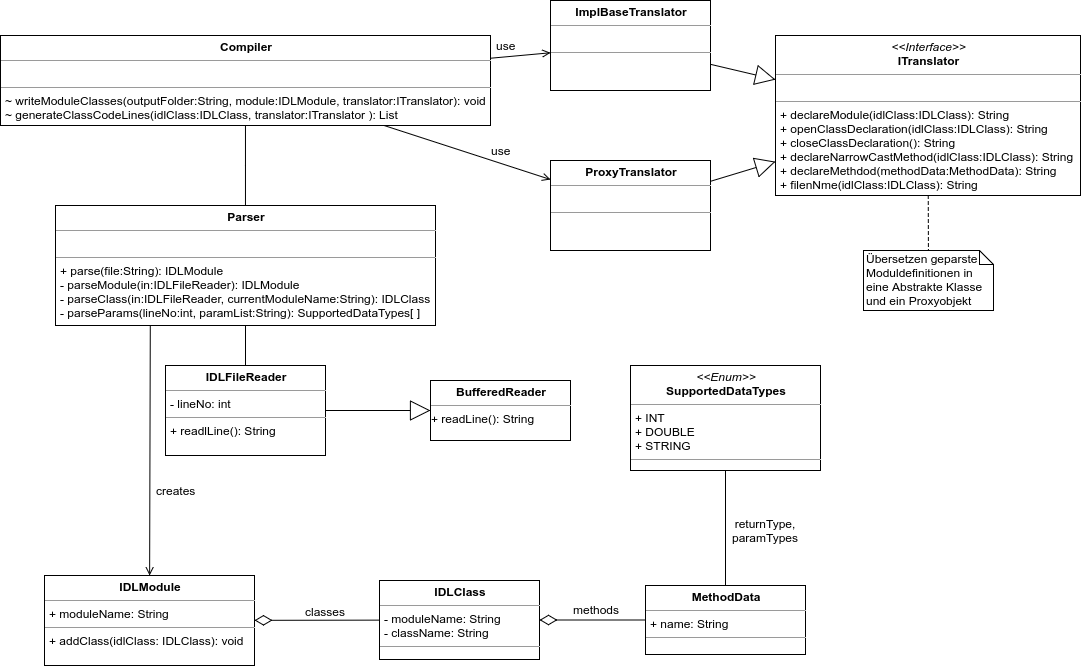
\includegraphics[width=\textwidth]{Compiler_FDM.png}
    \caption[fdm-compiler]{Fachliches Daten Modell des IDL-Compilers}
    \label{fig:fdm-compiler}
\end{figure}

Der Compiler besteht aus vier Komponenten (siehe Abbildung \ref{fig:compiler-component-diagram}). In der
Hauptkomponente (Compiler) ist der eigentliche Compiler mit seiner Mainmethode. Diese wird nach außen frei gegeben.

Der Compiler benutzt den Parser um eine IDL-Datei zu parsen und daraus ein IDLModule zu erstellen (siehe Abbildung
\ref{fig:fdm-compiler}). Diese IDLModule beinhaltet alle Klassen. Jede Klasse hat eine Ansammlung von Methoden.
Der Compiler schreibt nachdem die IDL-Datei geparsed wurde alle erkannten Klassen im Modul der IDL-Datei mit Hilfe der
Translator an den angegeben Ausgabepfad.\\

Die Translator haben ein fest definiertes Interface. Dadurch können leichter neue Translator erstellt werden und
Translator ausgetauscht werden. Außerdem ist dadurch der Übersetzungsprozess logisch von der Syntax der zu übersetzenden
Klasse getrennt.
Es gibt insgesamt zwei Translators. Einen um die Stubs (ImplBase) zu erstellen und einen
um die Proxy Klassen zu erstellen. Die Translators sind also dafür zuständig die IDLModules zu kompilieren in die
gewünschten Java Klassen.\\

Die Parser Komponente und die IDLModel Komponente wurden mit Hilfe der vorgegeben Klassen aus der Aufgabe erstellt und
erweitert.

\subsection{mware\_lib}
\subsubsection{Aufgabe und Verantwortung}
Die Bibiothek mware\_lib stellt die Middleware für entfernte Methodenaufrufe dar. Sie ist vergleichbar mit einem ORB in
einer CORBA Umgebung. Sie ist dafür zuständig, über den NameService Objekte über einen Namen anzusprechen und die
Methoden der Objekte auf einem entfernten Server aufzurufen. Außerdem müssen Server mit Hilfe der Middleware Objekte im
NameService anmelden können.

Die Middleware muss also vom Client und dem Server eingebunden werden.

\subsubsection{Schnittstelle}
\begin{lstlisting}
public class ObjectBroker {
    /**
     * Main entry point to the middleware.
     *
     * @param serviceHost String host of NameService
     * @param listenPort  int Port of NameService
     * @param debug       boolean indicates extra logging
     * @return ObjectBroker
     */
    public static ObjectBroker init(String serviceHost, int listenPort, boolean debug);

    /**
     * Returns the NameService (proxy Object / Client).
     *
     * @return NameService
     */
    public NameService getNameService();

    /**
     * Initiates the shutting down sequence for the middleware.
     */
    public void shutDown();
}

/**
 * Interface for communication between ObjectBroker
 */
public class Communication {
    /**
     * Invokes a method for a given Object and returns the result
     *
     * @param ref       ObjectReference of the method
     * @param method    String method name
     * @param args      Object.. arguments of the method
     * @return Object result of the called method
     */
    public Object invoke(ObjectReference ref, String method, Object.. args);

    /**
     * Starts the receiver
     */
    public void startReceiver();

    /**
     * Handles incoming requests, calls function locally and answers request
     *
     * @param clientSocket    Socket from incoming client
     */
    public Runnable handleIncomingRequest(Socket clientSocket);
}
\end{lstlisting}

\subsubsection{Entwurfsentscheidungen}
\begin{figure}[H]
    \centering
    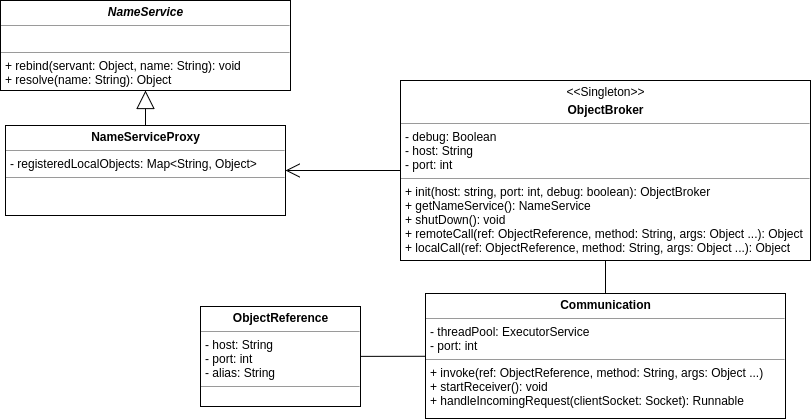
\includegraphics[width=\textwidth]{Middleware_FDM.png}
    \caption[fdm-middleware]{Fachliches Daten Modell der Middleware}
    \label{fig:fdm-middleware}
\end{figure}

Der ObjectBroker wird gemäß Vorgabe in einer statischen Methode initialisiert. Außerdem wird er mit dem
Singleton Pattern realisiert. Server und Client Anwendungen interagieren über den ObjectBroker mit der Middleware.
Der ObjectBroker kann also zum Einen im Server Kontext und zum Anderen im Client Kontext benutzt werden.\\

In der Communication Komponente der Middleware ist das Communication Modul. Dieses Modul ist für die Kommunikation
zwischen verschiedenen Instanzen der Middleware zuständig (GIOP).
Der Hostname des Servers wird nicht direkt übergeben, sondern per Java - API
dynamisch ermittelt. Wir behalten uns vor, für das Praktikum ein Netzwerkinterface anzugeben.
Die Kommunikation wird über den Port 9002 via TCP geführt. 

Dazu wird die Anfrage des entfernten Methodenaufrufes eines Objektes an das Communication Modul der Middleware des
Servers gesendet. Die Antworten werden als Objekte an den anfragenden Client zurückgeschickt.

Wenn eine Methode aufgerufen wird, die nicht im entfernten Objekt exisitert, sendet das Communication Modul des Servers
als Antwort eine RuntimeException an das CommunicationModul der Middleware des aufrufenden Clients.\\

Das Communication Modul ist ein nebenläufiger Prozess, der startet, sobald der ObjektBroker initalisiert wird
(\texttt{startReceiver}). Pro eintreffende Client Anfrage wird ein neuer Prozess gestartet
(\texttt{handleIncomingRequest}), der die Anfrage bearbeitet und beantwortet. Dazu wird das ObjectBroker Singleton
aufgerufen, um die Methode für das ObjectReference - Objekt lokal auszuführen (\texttt{localCall} im ObjectBroker).\\
ObjectReference ist Teil des Nameservice - Protokolls und im Abschnitt 'Protokolle' näher beschrieben.

Ausgehende Anfragen vom Communication Modul werden durch die Schnittstellenmethode \texttt{invoke} ausgeführt.
Dabei wird die Anfrage an den Server gesendet, der aus der ObjectReference ersichtlich ist. Die Antwort der Anfrage
wird dann als Objekt gelesen und weitergeleitet. Die Anfrage kann dabei mit einer RuntimeException beantwortet werden.
Diese wird durch das Communication Modul dann einfach an die aufrufende Komponente weitergeleitet.

Falls keine Antwort kommt (clientTimeout - 10s), wird auch eine RuntimeException an die aufrufende Komponente
weitergeleitet.\\

Der ObjectBroker beinhaltet zusätlich einen Client für den NameService in der NameService Komponente. Dieser sendet
Nachrichten über das NameServiceProtocol (siehe Abschnitt \ref{nameservice-entwurf}). Er empfängt serialisierte
ObjectReference Objekte. Er implementiert die clientseitigen Methoden für \texttt{resolve} und \texttt{rebind}.

Den Hostnamen und den Port des NameService Servers bekommt er durch den ObjectBroker weitergereicht
(\texttt{init} des ObjectBrokers). Der NameService wird durch den ObjectBroker also erstellt und ist in diesem
referenziert. Der NameService beinhaltet zusätzlich eine Map, in der lokale Objekte mit einem Namen hinterlegt sind.
Bei einem \texttt{rebind} werden die Objekte zusätzlich in dieser Map registriert.
Diese lokale Registry wird für einkommende Anfragen eines entfernten Methodenaufrufes verwendet. Mit dieser lokalen
Registry können dann die Namen in lokale Objekte aufgelöst werden, die dann zum Ausführen der Methoden verwendet werden.
Die lokale Registry ist threadsafe, damit parallele Anfragen bearbeitet werden können.\\

Der ObjectBroker an sich ist ein Singleton, das eine Referenz zum Communication Modul und zum NameService (Proxy) hält.
Ein entfernter Methodenaufruf wird über die vom Compiler erstellten Klassen ausgeführt.

Dafür wird zunächst mit Hilfe des NameService des ObjectBrokers per \texttt{resolve} die ObjectReference geholt. Diese
wird per \texttt{narrowCast} in ihr Stellvertreterobjekt transformiert (Proxy). Dieses Stellvertreterobjekt leitet alle
Methodenaufrufe an die \texttt{remoteCall} Methode des ObjectBrokers weiter. Dieser delegiert das an sein Communication
Modul, das die Antwort an den ObjectBroker zurückgibt. Der ObjectBroker gibt die Antwort dann an das
Stellvertreterobjekt weiter. Diese Antwort kann eine RuntimeException sein.

Ein lokaler Methodenaufruf wird vom Communication Modul an den ObjectBroker gesendet. Der ObjectBroker löst den Namen
mit seinem NameService in ein lokales Objekt auf und führt die Methode auf diesem aus, wenn sie vorhanden ist. Das
Ergebnis der Methode wird an das Communication Modul weitergeleitet. Ansonsten wird eine RuntimeException an das
Communication Modul weitergeleitet.\\

Bei einem \texttt{shutdown} im ObjectBroker wird das Communication Modul gestoppt (\texttt{stopReceiver}) und die
eigene Referenz des ObjectBrokers im ObjectBroker auf das leere Element gesetzt (wegen Singleton).

\subsubsection{Konfigurationsparameter}

\begin{itemize}
    \item Host, der Hostname des entfernten NameService
    \item Port, der Port des entfernten NameService
	\item Debug, boolean konfiguriert, ob debug Nachrichten geloggt werden sollen
\end{itemize}

\section{Protokolle}
\subsection{Nameservice-Protokoll}
Alle Protokolle die der Nameservice verwendet, sind in einer externen Bibliothek implementiert.
Dies schließt das Protokoll für Methodenaufrufe des Nameservice, und das serialisierbare
ObjectReference-Objekt mit ein.

Für Methodenaufrufe (rebind / resolve) empfängt der Nameservice Nachrichten im folgenden Format:
\begin{itemize}
\item Byte 0: Art des Befehls. (0 = Rebind, 1 = Resolve)
\item Byte 1 - 11: Alias für rebind / resolve
\item Byte 12 - n: Serialisiertes Referenz Objekt (ObjectReference), nur für rebind benötigt
\end{itemize}

Nachrichten dieser Form können mit statischen Methoden in der Klasse NameServiceProtocol generiert werden.

Das serialisierte Referenzobjekt (ObjectReference) enthält Hostname, Port und Alias (im Nameservice hinterlegte Namensreferenz) des 
entfernten Objektes.

\subsection{Protokoll für entfernte Methodenaufrufe}

Das Protokoll für entfernte Methodenaufrufe ist als serialisiertes Objekt in der Klasse 
RemoteCall (teil der Middleware) implementiert. Es enthält den Alias des aufzurufenden Objektes,
sowie Name und Argumente der aufzurufenden Methode.
In diesem Protokoll kommunizieren der Client mit dem Server.
Rückgabewerte des Servers werden ohne Protokoll als serialisierte Objekte geschickt.
\end{document}